\documentclass[a4paper,10pt]{article}
\usepackage[utf8]{inputenc}
\usepackage{amssymb}
\usepackage{amsfonts}
\usepackage{amsmath}
\usepackage{enumerate}
\setlength{\parindent}{0pt}
\usepackage[margin=1in]{geometry}

\usepackage{graphicx}
\graphicspath{ {./images/} }

\usepackage{listings}
\usepackage{color}

\definecolor{dkgreen}{rgb}{0,0.6,0}
\definecolor{gray}{rgb}{0.5,0.5,0.5}
\definecolor{mauve}{rgb}{0.58,0,0.82}

\lstset{frame=tb,
  language=C++,
  aboveskip=3mm,
  belowskip=3mm,
  showstringspaces=false,
  columns=flexible,
  basicstyle={\small\ttfamily},
  numbers=none,
  numberstyle=\tiny\color{gray},
  keywordstyle=\color{blue},
  commentstyle=\color{dkgreen},
  stringstyle=\color{mauve},
  breaklines=true,
  breakatwhitespace=true,
  tabsize=3
}
\begin{document}

Jason Qiu

CS 385 Homework Assignment $\#3$

\emph{I pledge my honor that I have abided by the Stevens Honor System.}
\begin{enumerate}
\item Below is the matrix:

\begin{tabular}{|c||c|c|c|c|c|c|c|c|c|c|}
	\hline
	x & 1 & 2 & 3 & 4 & 5 & 6 & 7 & 8 & 9 & 10\\
	\hline
	\hline
	1 & 0 & 1 & 0 & 1 & 0 & 0 & 0 & 0 & 0 & 0\\
	\hline
	2 & 0 & 0 & 0 & 0 & 1 & 0 & 0 & 0 & 0 & 0\\
	\hline
	3 & 0 & 0 & 0 & 0 & 1 & 0 & 0 & 0 & 0 & 0\\
	\hline
	4 & 0 & 1 & 0 & 0 & 0 & 0 & 0 & 0 & 0 & 0\\
	\hline
	5 & 0 & 0 & 0 & 1 & 0 & 0 & 0 & 0 & 1 & 0\\
	\hline
	6 & 0 & 0 & 0 & 0 & 0 & 1 & 0 & 1 & 0 & 0\\
	\hline
	7 & 0 & 0 & 0 & 0 & 1 & 0 & 0 & 0 & 0 & 0\\
	\hline
	8 & 0 & 0 & 0 & 0 & 0 & 0 & 0 & 0 & 0 & 0\\
	\hline
	9 & 0 & 0 & 0 & 0 & 0 & 0 & 1 & 0 & 0 & 1\\
	\hline
	10 & 0 & 0 & 1 & 0 & 1 & 0 & 0 & 0 & 0 & 0\\
	\hline
	\end{tabular}
\item \{\{2, 4\}, \{5\}, \{5\}, \{2\} \{4, 9\}, \{6, 8\}, \{5\}, \{\}, \{7, 10\}, \{3, 5\}\}

\item 1, 2, 4, 5, 9, 7, 10, 3, 6, 8

\item 1, 2, 5, 4, 9, 7, 10, 3, 6, 8

\item \begin{enumerate}[(a)]
	\item $\mathcal{O} (V^2)$

	\item $\mathcal{O} (V+E)$
\end{enumerate}

\item \begin{enumerate}[(a)]
	\item $\mathcal{O} (V^2)$

	\item $\mathcal{O} (V+E)$
\end{enumerate}


\item If a graph has few edges ($E < V$), an adjacency matrix contains a lot of unnecessary 0's that an adjacency list would not have.

\item If we detect a visited node that isn't the parent in an undirected graph, we have a cycle.

\item No. Below is a graph for which BFS finds the cycle first:

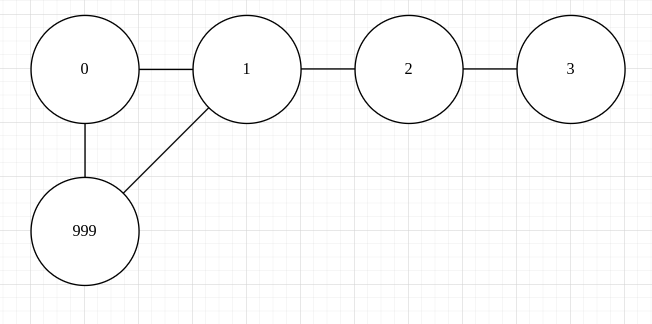
\includegraphics[scale=0.25]{hw3_fig1}

And below is a graph for which DFS finds the cycle first:

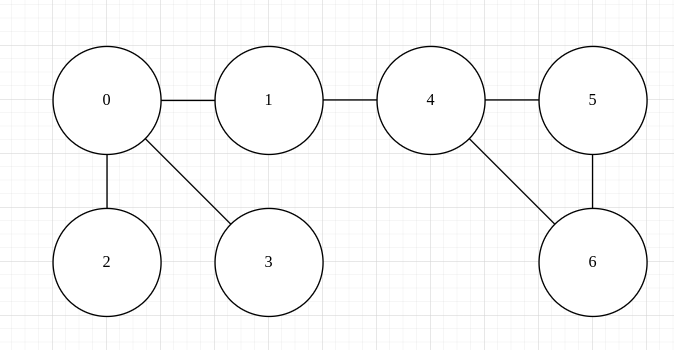
\includegraphics[scale=0.25]{hw3_fig2}

\item There contain multiple cycles in the graph on the top,  meaning multiple nodes will never have indegree 1 and therefore will not be sorted.

\item 1, 6, 4, 8, 2, 5, 9, 7, 10, 3

\end{enumerate}
\end{document}